\documentclass{article}

\usepackage[letterpaper,top=2cm,bottom=2cm,left=3cm,right=3cm,marginparwidth=1.75cm]{geometry}

\usepackage{amsmath, amsfonts, amssymb}
\usepackage{graphicx}
\usepackage{algorithm}
\usepackage[noend]{algpseudocode}
\usepackage{amsthm}
\usepackage{bm}
\usepackage{cases}
\usepackage{caption}
\usepackage{hyperref}

\DeclareMathOperator*{\argmin}{argmin}


\usepackage{setspace}
\onehalfspacing

\usepackage{soul}
\usepackage{xcolor}
\def\elr#1{{\color{cyan}\textbf{ELR:[#1]}}}
\def\apg#1{{\color{red}\textbf{APG:[#1]}}}
\def\bwr#1{{\color{violet}\textbf{BWR:[#1]}}}

\usepackage{natbib}
\bibliographystyle{unsrtnat}


\title{Evaluating infectious disease forecasts with allocation scoring rules}
\author{Aaron Gerding, Nicholas G. Reich, Benjamin Rogers, Evan L. Ray}

\begin{document}

\newcommand{\del}[2]{\frac{\partial {#1} }{\partial {#2}} }
\newcommand{\dby}[2]{\frac{d {#1} }{d {#2}} }
\newcommand{\sbar}{\overline{s}}
\newtheorem{proposition}{Proposition}

\theoremstyle{remark}
\newtheorem*{remark}{Remark}

\maketitle

\begin{abstract}

The COVID-19 pandemic has led to rapid innovation in methods for eliciting and evaluating forecasts of infectious disease burdens, with a primary goal being to help public health workers make informed decisions about how to manage these burdens. However, explicit descriptions or quantifications of the value forecasts add to society through the decisions they support are elusive.  Moreover, there has only been limited discussion of how predominant forecast evaluation metrics might indicate the success of policies based in part on those forecasts.

Here we pursue one possible tether between multivariate forecasts and policy: the allocation of limited medical resources in response to COVID-19 hospitalizations in various regions so as to minimize expected unmet need. Given probabilistic forecasts of hospitalizations in each region, we formulate an allocation algorithm following techniques developed in operations research. We then score forecasts according to how much unmet need their associated allocations would have allowed. We illustrate this scheme with quantile forecasts of COVID-19 hospitalizations in the US at the state level that are recorded in the COVID-19 Forecast Hub, with the goal of determining the allocation of a hypothetical limited resource across the states. The forecast skill ranking given by this allocation scoring rule can vary substantially from the ranking given by the weighted interval score now used by the CDC, especially during surges in hospitalizations such as in late 2021 as the Omicron wave began. We see this as strong evidence that the allocation scoring rule detects forecast value that is missed by traditional accuracy measures and that the general strategy of designing scoring rules that are directly linked to policy performance is a promising research direction for epidemic forecast evaluation.

\end{abstract}

\section{Introduction}

%High level points to cover in introduction:
%\begin{itemize}
%\item People are using infectious disease forecasts as an input to decision making
%\item There are standard ways to evaluate forecasts that are responsive to decision making context, and use of those methods is relatively common in other fields like economics and meteorology
%\item However, there's not much work in infectious disease that does this
%\item In practice, infectious disease forecasts have typically been evaluated with "off the shelf" scoring rules such as the WIS which is an approximation to CRPS, log score, and so on.
%\item In this work, our goal is to begin to address that gap. We focus on a resource allocation setting.
%\item There is past work focusing on resource allocation in the operations research literature, but it doesn't take the step of getting to a measure of forecast skill.
%\item That is, while there is plenty of work on
%\begin{itemize}
%\item DM under risk, where probabilities are taken as known and expected utility is maximized
%\item DM under uncertainty, where probabilities are taken as unknown and robust (i.e. maximin) decisions are sought
%\end{itemize}
%little seems to have been said on how forecasts can be evaluated by how well they convert a problem of DM under uncertainty to a problem of DM under risk.
%\end{itemize}

% People using infectious disease forecasting as an input to decision making:

%Center for Forecasting and Outbreak Analytics (CDC) https://www.cdc.gov/forecast-outbreak-analytics/annual-report/2023/key-accomplishments.html#omicron-response anual report
%  Bertsimas gives data-driven approach to provide clincal insights and support ventilator allocation for policy makers,

% "Our results have been used at the clinical level by several hospitals to triage patients, guide care management, plan ICU capacity, and re-distribute ventilators. At the policy level, they are currently supporting safe back-to-work policies at a major institution and vaccine trial location planning at Janssen Pharmaceuticals, and have been integrated into the US Center for Disease Control’s pandemic forecast."


%https://www.cdc.gov/mmwr/preview/mmwrhtml/su6303a1.htm


Infectious disease forecasting models have emerged as important tools in public health. Predictions of disease dynamics have been used to inform decision-making about a wide variety of measures to reduce disease spread and/or mitigate the severity of disease outcomes. For example, estimates of expected onset of flu season have been used to aid national vaccination strategies \citep{igboh2023timing}, and forecasts of Ebola dynamics have been used to allocate surveillance resources \citep{meltzer2014estimating, rainisch2015regional}. \cite{bertsimas2021predictionsCOVID} developed tools to inform decision making from infectious disease forecasts, which have been used to inform allocation of limited medical supplies such as ventilators, ICU capacity planning, and vaccine distribution strategy. Models developed by \cite{fox_real-time_2022} have been used to inform resource and care site planning, as well as community guidelines for masking, traveling, dining and shopping (University of Texas, 2022) \nocite{utnews2022}. In April of 2022, the Centers for Disease Control and Prevention (CDC) announced the launch of the Center for Forecasting and Outbreak Analytics (CFA) to translate disease forecasts into decision-making (CDC, 2022)\nocite{cdc2022cfa}, indicating that this has been identified as an important direction at the highest levels of government public health response. The value of infectious disease forecasts has typically been measured by how closely they predict disease outcomes such as cases, hospitalizations or deaths using, for example, root mean square error (RMSE) \citep{papastefanopoulos2020covid} or weighted interval score (WIS) \citep{bracher2021evaluating}, however, recently authors have been calling for evaluating forecasts through their impact on policy \citep{marshall2023predictions}.

In decision-making settings where it is possible to quantify the utility or loss associated with a particular action, standard tools of decision theory provide a procedure for developing forecast scoring rules that measure the value of forecasts through the quality of the decisions that they lead to. We give an overview of these procedures in Section \ref{sec:methods.decisiontheory}. There is a large history of literature applying these ideas to obtain measures of the value of forecasts that are tied to a decision-making context, primarily in fields such as economics and finance, supply chain management, and meteorology. We review this work only briefly here, and we refer the reader to \cite{yardley2021utility_cost_forecasts} for a general overview, and to \cite{pesaran2002decision_based_eval} and \elr{TODO: identify relevant review or book style summary for meteorology} for discussions focused on applications to economics and meteorology, respectively. In finance, the value of forecasts can often be measured by the profits generated by trading decisions informed by the forecasts, perhaps adjusted for risk levels \cite[e.g.,][]{leitch1991economicForecastEval, cenesizoglu2012returnPredictionEconValue}. In applications to supply chain management and meteorology, the value of forecasts has typically been operationalized by considering the costs associated with decisions regarding the amount of inventory to hold or the level of protection against the impacts of extreme weather events to enact {Peter Catt (2007), Fotios Petropoulos and colleagues (2019), Nada Sanders and Gregory Graman (2009), T.N. Palmer (2002), Florian Pappenberger and colleagues (2015)}. For example, in supply chain management these decisions may incur costs related to holding inventory, labor, or providing poor service, while in meteorology we may need to balance the costs of implementing protective measures with the costs of potentially preventable weather damages. In this framework, a forecast has value if it leads to decisions with low total costs. In all of these fields, analyses have consistently found that common measures of statistical forecast accuracy do not necessarily correspond directly to measures of the value of forecasts as an input to decision-making \cite[e.g.,][]{leitch1991economicForecastEval, cenesizoglu2012returnPredictionEconValue}. % Consistently, but not uniformly

% Other important early contributions include Nelson (1972) and White (1966), who are amongst the first to consider the problem of forecast evaluation from the perspective of decision theory and dynamic programming. Nelson, in particular, articulates the concept of the “value of a (probability) fore- cast” to an individual decision-maker as the expected value of his/her payoff using the probability forecasts relative to the payoff expected if unconditional probability estimates are used.

% This has been somewhat rectified during the last decade as the observation that financial series are predictable has led to an attempt to understand the economic significance of this finding. See, for example, Breen, Glosten, and Jagannathan (1989), Leitch and Tanner (1991), McCulloch and Rossi (1990), West, Edison, and Cho (1993), Pesaran and Timmermann (1994, 1995), Satchell and Timmermann (1995), and Skouras (1998).

% Theil (1960), White (1966)

However, we are aware of only a limited body of work that explicitly attempts to measure the value of infectious disease forecasts through their impact on policy, and much of this discussion has proceeded informally. For example, \cite{ioannidis2022forecastingCOVIDfailed} discuss the possible negative consequences of inaccurate forecasts of infectious disease, but do not attempt to quantify the utility or loss incurred as a result of those forecasts. Separately, there is a thread of literature that does quantify the link between infectious disease modeling and policy making, but this work has been done outside of a forecasting context. As an example, \cite{Probert2016decisionMakingFootMouth} develop measures of the cost of actions designed to control a hypothetical outbreak of foot-and-mouth disease and use this framework to explore policy recommendations from a variety of simulation-based projection models.

In practice, probabilistic infectious disease forecasts have most often been made for observations that emerge from public health surveillance systems and have typically been evaluated with standard, ``off-the-shelf'' scoring rules.
For example, seasonal influenza forecasts in the US and dengue forecasts for Peru and Puerto Rico targeted public health surveillance measures of incidence over time and space, and used log-score and mean absolute errors to evaluate forecast skill \citep{mcgowan_collaborative_2019,reich_collaborative_2019,johansson_open_2019}.
Pandemic COVID-19 forecasts of observed cases, hospitalizations and/or deaths in the US and Europe, as reported by municipal, state, or federal surveillance systems, were evaluated using the weighted interval score (WIS, which is an approximation of the continuous ranked probability score, or CRPS), and prediction interval coverage \citep{cramer_evaluation_2022,fox_real-time_2022,sherratt2023predictive}.
Similarly, CRPS was also used to assess probabilistic forecasts of dengue incidence at the district level in Vietnam \citep{colon-gonzalez_probabilistic_2021}.
While some of these scores can be interpreted through the lens of decision theory, and all of the application-specific papers cited above had authors from public health agencies, none of them make explicit connections between forecast evaluation and how a forecast was used in practice.

In this work, we begin to fill this gap between the ways that infectious disease forecasts have traditionally been evaluated and the ways that they have been used to support public health policy.
We consider a setting in which forecasts are used to help determine the allocation of a limited quantity of medical supplies across multiple regions.
We define a new forecast scoring rule --- the {\em allocation score} --- that evaluates forecasts based on how beneficial resource allocations derived from them would turn out to be.
%Unlike the traditional measures of forecast skill such as WIS, CRPS, and log score, the proposed allocation score measures the suitability of a forecast as an input to this specific decision making task.

Briefly, the allocation score of a forecast is the avoidable unmet need that results from using that forecast to set resource allocations by minimizing expected unmet need.
For example, suppose that a decision-maker is provided with forecasts of the level of need for medical resources in each of several states or hospital systems.
If there is a limited amount of the medical resource that is available to distribute, a decision-maker could choose an allocation of that resource across locations that minimizes the expected unmet need according to that forecast.
As measured by the allocation score, one forecast is better than another if it would lead decision-makers to an allocation that results in less unmet need.
%By ``unnecessary'' we mean the unmet need that could have been avoided by an oracle that knows exactly how much need will occur in each location and divides the amount $K$ so that nothing is wasted in one location while it could be put to use in another.
If the amount of resources that is available to distribute is less than the actual need, some amount of unmet need is unavoidable.
The allocation score for a forecast does not include the unmet need that was unavoidable given the resource constraint, and so it measures only the amount of unmet need that could have been prevented by using a different allocation of available resources than that suggested by the forecast.
We elaborate on these ideas in Section~\ref{sec:methods}.

We present an illustrative analysis using the allocation score to evaluate forecasts of hospital admissions in the US leading up to the Omicron wave in winter 2022.
This analysis is ``synthetic'' in that it does not correspond to an actual analysis that supported decision-making in real-time.
However, the framework described in this paper corresponds to real-world decisions that must be made by public health administrators around the globe, and could be adapted in the future for such real-time situations.
For example, forecasts for districts in Sierra Leone of bed demand to care for patients with Ebola was the subject of a real-time modeling study in late 2014 and early 2015 \citep{camacho2015-ebola-bed}.
And, in 2020, a model developed by an academic research group turned predictions of COVID-19 hospitalizations into estimates of ventilator usage and and shortages. This framework was used by the Hartford HealthCare system in Connecticut ``to align ventilator supply with projected demand at a time where the [COVID-19] pandemic was on the rise'' \citep{bertsimas2021predictionsCOVID}.
These examples illustrate the potential for forecasts to inform decisions about how to allocate limited supplies such as temporary hospital beds, ventilators, personal protective equipment, or other supplies that are known to be effective at reducing transmission or severity of disease.
However, we emphasize again that these studies did not take the step of evaluating forecasts based on the quality of the allocation decisions that they supported or could have been used to support.

% As described above, there exists both a rich literature on outbreak forecast evaluation and an emerging body of work on turning forecasts into resource allocation decisions. 
% However, we have not found literature exploring whether standard forecast accuracy metrics are sufficient for evaluating how well forecasts support allocation decisions.

% \subsection{Organization}

The remainder of this article is organized as follows. 
In Section \ref{sec:methods}, we review the general framework for developing scoring rules for probabilistic forecasts using the tools of decision theory, develop a novel scoring rule that is motivated by the problem of allocating limited medical supplies, and explore the relationship between the proposed allocation score and existing scoring rules such as CRPS. 
In Section \ref{sec:application} we illustrate the scoring rule through an application to short-term forecasts of COVID-19 hospital admissions in the US. 
Section \ref{sec:discussion} summarizes our contributions and discusses opportunities for further extensions in future work.

\section{Methods}
\label{sec:methods}

We begin with an informal description of the allocation score and some examples illustrating its key characteristics in section \ref{sec:methods.overview}. In section \ref{sec:methods.detailed} we develop the allocation score more carefully, building on decision-theoretic procedures for deriving proper scoring rules. We then comment on some connections between the allocation score that we propose and other common scores that can be derived from decision-theoretic foundations, such as the quantile score, WIS, and CRPS, in section \ref{sec:methods.related}.

\subsection{Overview of Allocation Scoring}
\label{sec:methods.overview}

Suppose that a decision-maker is tasked with determining how much of a resource such as a medical supply should be allocated to each of $N$ locations, subject to the constraint that only $K$ units of the resource are available.
If the decision-maker is provided with a multivariate forecast $F$ that predicts resource need in each location, one option is to choose the resource allocation that minimizes the expected total unmet need according to the forecast.
We will give a more precise mathematical statement in section \ref{sec:methods.allocation}, but informally, the total expected unmet need according to the forecast is
\begin{align}
\sum_{i=1}^N E_{F_i}[\text{unmet need in location $i$}], \label{eqn:informal_objective}
\end{align}
where $F_i$ is the marginal forecast distribution of need in location $i$ and the unmet need in a particular location is the difference between resource need in that location and the number of resources that were allocated there.
This allocation problem has an intuitively appealing solution: allocate so that the probabilities of need exceeding allocation in various locations are as close to each other as possible.
This will lead to the allocations provided by $F$ being quantiles of the marginal distributions $F_i$ for some \emph{single} probability level $\tau$ that is shared in common for all locations.

After time passes and the actual level of resource need has been observed, the quality of a selected allocation can be measured by comparing the actual need in each location to the amount of resources that were sent there. Specifically, we compute the total unmet need that resulted from the selected allocation:
\begin{align}
    \sum_{i=1}^N \text{unmet need in location $i$}. \label{eqn:informal_loss}
\end{align}
We emphasize that in Equation \eqref{eqn:informal_loss} the calculation of unmet need is based on the actual resource need that was realized in each location, while in Equation \eqref{eqn:informal_objective} the calculation of unmet need was based on a hypothetical potential future level of resource need.
Once the actual levels of resource need have been observed, we can obtain a quantitative measure of the quality of alternative allocation decisions: one allocation is better than another if it results in lower total unmet need.

The \textbf{allocation score} of the forecast $F$ is the avoidable unmet need that results from using the allocation that minimizes the expected unmet need according to that forecast.
By ``avoidable unmet need'', we mean that the allocation score does not include the amount of unmet need that was inevitable simply because the amount of available resources $K$ was less than the need for resources.
Rather, the allocation score measures the unmet need that could have been avoided by an oracle that knows exactly how much need will occur in each location and divides the amount $K$ so that nothing is wasted in one location while it could be put to use in another. An allocation score of 0 is optimal, and indicates that no other allocation of resources could have met need better than the allocation suggested by $F$. A larger allocation score indicates that it would have been possible to improve upon the allocation suggested by $F$.

\paragraph{Example 1} Suppose we have a forecast $F$ for need in two locations with $F_1 = \mathrm{Exp}(1 / \sigma_1)$ and $F_2 = \mathrm{Exp}(1 / \sigma_2)$, where $\sigma_1 = 1$ and $\sigma_2 = 4$. When the marginal forecasts are exponential distributions, it can be shown that the optimal allocation divides the available resources among the locations proportionally to the scale parameters $\sigma_i$ (see section *** of the supplemental materials). If we have $K = 5$ units of our resource available, the optimal allocation according to $F$ would be 1 unit of resources in location 1 and 4 units of resources in location 2. If, on the other hand, we have $K = 10$ units available, we will allocate 2 units of resources to location 1 and 8 units to location 2. Figure~\ref{fig:exp_alloc_example} illustrates the situation.

\begin{figure}
    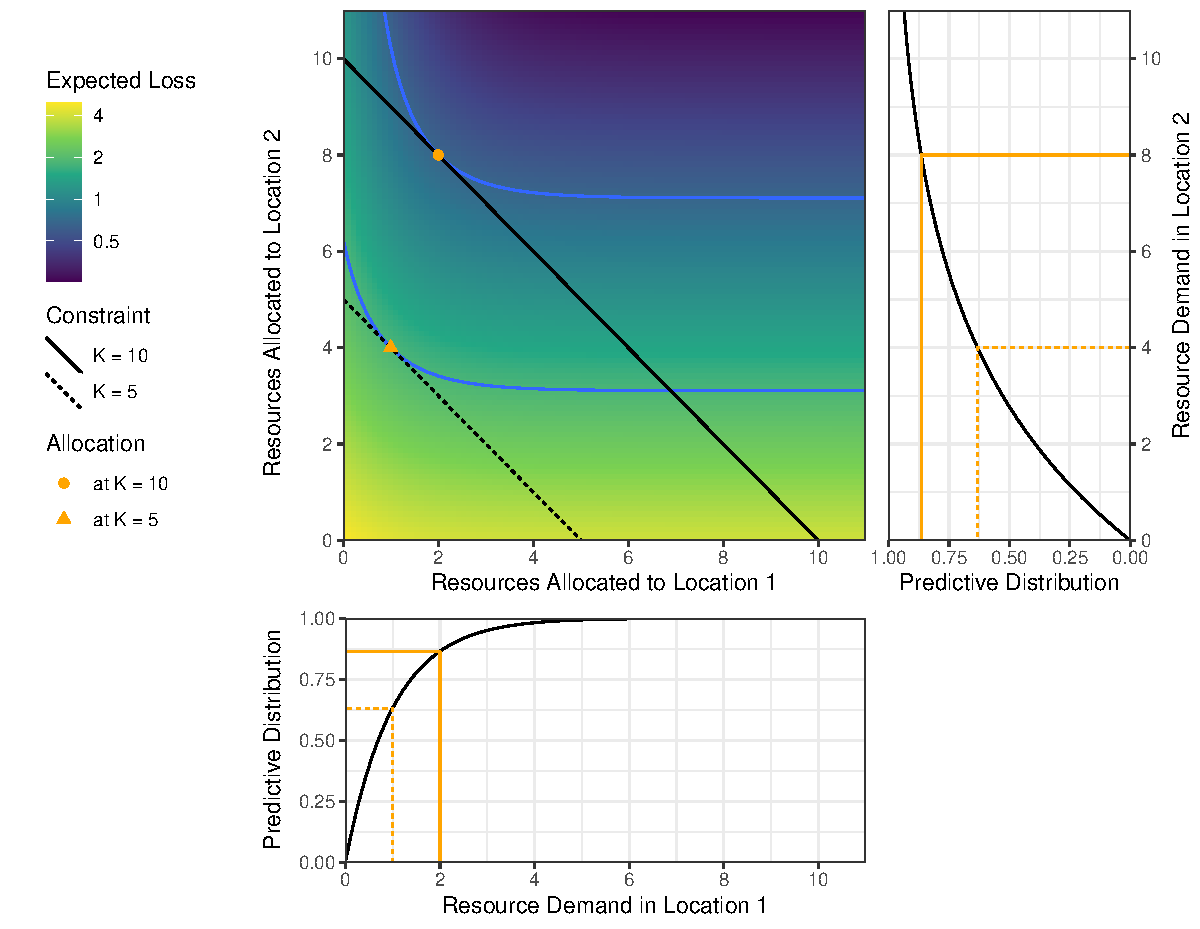
\includegraphics[width=\textwidth]{../figures/exponential_pred_expected_loss.pdf}
    \caption{An illustration of the resource allocation problem in Example 1. There are $N = 2$ locations, with predictive distributions $F_1 = \mathrm{Exp}(1)$ and $F_2 = \mathrm{Exp}(1/4)$. The cdfs of these distributions are illustrated in the panels at bottom and right. In the center panel, the background shading corresponds to the expected loss according to these forecasts. Diagonal black lines indicate resource constraints at $K=5$ and $K=10$ units; any point along those lines corresponds to an allocation that meets the resource constraint. For these forecasts, the optimal allocations are $(1, 4)$ for $K=5$ and $(2, 8)$ at $K=10$. These allocations are at the point on the constraint line where the expected loss is smallest, which also corresponds to the point where a level set of the expected loss surface (blue curve) is tangent to the constraint.}
    \label{fig:exp_alloc_example}
\end{figure}

Next suppose that we observe needs of 1 and 10 in locations 1 and 2, respectively.
Based on these observed needs, we can measure the quality of the allocation suggested by the forecast by calculating the amount of unmet need that resulted from that allocation over and above what was unavoidable given the resource constraint.
With $K = 5$ units of the resource, the allocation based on the forecast exactly meets the observed need in location 1, but it leaves 6 units of need unmet in location 2.
However, working within the resource constraint, no other allocation could have done better: for example, allocating 0 units of resources to location 1 and 5 to location 2 still results in a total unmet need of 6 across both locations. Therefore, the forecast's allocation score is 0 with $K = 5$.
On the other hand, when $K = 10$, the forecast $F$'s allocation results in $10 - 8 = 2$ units of unmet need in location 2 despite leaving no need unmet in location 1.
In this case, the oracle would be able to prevent all but 1 of the total 11 units of need from going unmet, for example by allocating 1 unit of resources to location 1 and the remaining 9 units of resources to location 2.
The allocation score for the forecast when $K = 10$ would therefore be 1 (= 2 realized $-$ 1 unavoidable) in units of avoidable unmet need.

These scores illustrate a general result: allocation scores for a forecast will tend to be larger when the resource constraint is close to the observed need, because this is when it matters most which locations are allocated more or less resources. If the resource constraint is very small, any allocation of those limited resources will result in a large amount of unmet need. If the resource constraint is very large, it becomes less important which locations receive relatively more or less resources because all locations will receive enough resources to meet their need.

\paragraph{Example 2} Now consider a different forecast that also has exponential distributions for resource need in each location, but that has the scale parameters $\sigma_1 = 2$ and $\sigma_2 = 8$, twice as large as the scale parameters of the forecast in Example 1. Because the optimal allocation is proportional to the scale parameters, this forecast would lead to the same optimal allocations as the forecast in Example 1, and would therefore be assigned the same allocation score.

Note the way in which these forecasts incurred a positive (i.e., non-optimal) allocation score of 1 when $K = 10$. It was not directly directly due to individual misalignments of the marginal forecasts $F_i$ with the observed needs, but rather because the allocations and observed needs were not proportional as vectors.
Restating: as far as allocation decisions are concerned, with a fixed constraint $K=10$ the fundamental problem with the forecast $F$ in Example 1 is not that it predicts a mean total resource need of $5$ units; it is that the realized need was 10 times as large in location 2 as in location 1, but the forecast only indicated that the resource allocation for location 2 should be 4 times the allocation for location 1.

This illustrates a fundamental property of the allocation score: at its core, it measures whether the forecast accurately captures the relative magnitudes of resource need across different locations, which is precisely the information that is needed to allocate resources to those locations subject to a fixed resource constraint.
On the other hand, the allocation score is not directly sensitive to whether the forecasts in each location correctly capture the magnitude of resource need in each individual location.
%For a given probability level $\tau$, if the quantiles $Q_i(\tau)$ of the marginal forecasts are proportional to the observed needs $y_i$, then the allocation score is zero for the resource constraint level $K = \sum Q_i(\tau)$.
This stands in marked contrast to other common scoring methods for multivariate forecasts that aggregate univariate scores such as CRPS or WIS for the marginal forecasts where a 
misalignment in one coordinate is penalized regardless of alignments in other coordinates. Note that we do not claim that the allocation score is generically preferable to these other scores \textemdash rather, it provides a view of forecast performance that is specifically tuned to the context of decision-making about resource allocations.

%It is therefore often straighforward to constuct forecasts $F$ and $\widetilde{F}$ for a given outcome distribution that switch rankings under the allocation and traditional scores by ensuring that the marginal forecasts of $F$ center sharply around allocations that are proportionally similar to the central tendencies of the outcome distribution but are strongly biased.

%While multivariate scoring rules have not seen wide application in infectious disease forecast evaluation, it seems that the allocation score would have a similar relationship with them, since while bias penalties in multi-variate scores can be offset by better forecasting of dependence structure, the proportional biases that allocation scoring are insensitive to are not \emph{per se} tolerated by multivariate scoring rules such as the energy score, variogram score, or Dawid-Sebastiani score. 

\subsection{A decision-theoretic development of the allocation score}
\label{sec:methods.detailed}

We give a high-level review of a general procedure for developing proper scoring rules that are tailored to specific decision-making tasks in section \ref{sec:methods.detailed.decisiontheory}, and then in section \ref{sec:methods.detailed.allocation} we apply that procedure to develop the allocation score based on the task of deciding on how to allocate a fixed supply of resources across multiple locations.

\subsubsection{The decision-theoretic setup for forecast evaluation}
\label{sec:methods.detailed.decisiontheory}

%In this section, we give an overview of the decision-theoretic setup for developing proper scoring rules that measure the value of a forecast as an input to decision making. We keep the discussion here at a somewhat informal level; we refer the reader to [some subset of Brehmer and Gneiting; Grünwald and Dawid; Dawid; Granger and Pesaran 2000; Granger and Machina 2006; Ehm et al. 2016] for more technically precise discussion.

In the framework of decision theory, a decision corresponds to the selection of an action $x$ from some set of possible actions $\mathcal{X}$. For example, $x$ may correspond to the level of investment in a measure designed to mitigate severe disease outcomes such as hospital beds, ventilators, medication, or medical staff, with $\mathcal{X}$ being the set of all possible levels of investment that we might select. The quality of a decision to take a particular action $x$ is measured in relation to an outcome $y$ that is unknown at the time the decision is made. For example, $y$ may correspond to the number of individuals who eventually become sick and would benefit from the mitigation measure, and informally, an action $x$ is successful to the extent that it meets the realized need. In the face of uncertainty, a decision-maker may use a forecast $F$ of the random variable $Y$ to help inform the selection of the action to take. We measure the value of a forecast as an input to this decision-making process by the quality of the decisions that it leads to.

We can formalize the preceding discussion with the following three-step procedure for developing scoring rules for probabilistic forecasts:
\begin{enumerate}
\item Specify a \emph{loss function} $s(x, y)$ that measures the loss associated with taking action $x$ when outcome $y$ eventually occurs.
\item Given a probabilistic forecast $F$, determine the \emph{Bayes act} $x^F$ that minimizes the expected loss under the distribution $F$.
\item The \emph{scoring rule} for $F$ calculates the score as the loss incurred when the Bayes act was used: $S(F, y) = s(x^F, y)$.
\end{enumerate}
%We use the letter $s$ for the loss function to align with the literature on evaluation of forecasts of continuous outcomes, in which context we can often identify the action $x$ with a functional (i.e., a numeric summary such as a mean or a quantile) of the forecast distribution $F$. In this context, $s$ may be used as a \emph{scoring function}. \elr{Consider moving preceding sentences to a footnote or just deleting them?}
This is a general procedure that may be applied in settings where it is possible to specify a quantitative loss function. Subject to certain technical conditions, scoring rules obtained from this procedure are proper. We refer the reader to [some subset of Brehmer and Gneiting; Grünwald and Dawid; Dawid; Granger and Pesaran 2000; Granger and Machina 2006; Ehm et al. 2016] for more technically precise discussion.

% , and we illustrate the ideas with two running examples: (1) some problem that results in quantile elicitation, (2) some allocation problem.

%A forecaster is asked to recommend, that is, \emph{predict}, the appropriate supply $x$ of some good or investment in some precautionary measure intended to satisfy a random future demand or need $Y$. As a running example, we will consider the provision of a limited supply of a limited health care resource such as oxygen or ventilators. Suppose there is an incremental loss $O \geq 0$ incurred when over-prediction leads to unused supply and an incremental loss $U > 0$ incurred when under-prediction leads to unmet demand or need.

% \subsection{A review of quantile score, CRPS, and the weighted interval score}
% \label{sec:methods.quantileloss}

% We review how the quantile score arises from a particular decision-making problem in section \ref{sec:methods.quantileloss.quantile}, and how CRPS can be obtained by integrating across values of the parameters of that decision-making problem, as well as the connection to WIS, in section \ref{sec:methods.quantileloss.crps}. These results have been thoroughly discussed in the literature [cite cite cite].

% \subsubsection{Decision-theoretic origins of the quantile score}
% \label{sec:methods.quantileloss.quantile}

% Suppose that a decision-maker is tasked with determining the quantity $x$ of a protective measure to procure; for example, $x$ might represent the number of hospital beds or amount of medicine to purchase. Additionally, suppose that each unit of this good has cost $C$ so that the total cost of procurement is $Cx$. The variable $y$ denotes the eventual realized need for this resource, e.g. the number of patients in need of a hospital bed or the amount of medication that is needed. We assume that each unit of unmet need incurs a loss denoted by $L$, so that if the selected procurement level $x$ is less than the realized need $y$, a loss of $L(x-y)$ results. At the time that a decision-maker determines the amount $x$ to procure, the demand $y$ is not yet known. We therefore define the random variable $Y$ that represents the as-yet-unknown level of demand. The forecast $F$ specifies a predictive distribution for $Y$. Here we identify $F$ with its cumulative distribution function (CDF), and $F^{-1}$ denotes the quantile function. With this formalization of the decision-making task, we can proceed to develop a proper scoring rule using the procedure outlined in section \ref{sec:methods.decisiontheory}.

% \paragraph{Step 1: specify a loss function.} Combining the cost of procuring goods at level $x$ with losses due to unmet need, we arrive at the overall loss function
% \begin{align}
% s_Q(x,y; C, L) = Cx + L(x-y)_-.
% \end{align}
% Here, $(x - y)_- := \max(-(x - y),0)$ is $0$ if the amount procured, $x$, is greater than or equal to the realized demand $y$; otherwise, it is $y - x$, the amount of unmet need.

% \paragraph{Step 2: Given a probabilistic forecast $F$, identify the Bayes act.} It can be shown that under the loss function $s_Q$, the Bayes act is a quantile of the forecast distribution at the probability level $\alpha = 1 - C/L$:
% \begin{align}
% x^F = F^{-1}(\alpha).
% \end{align}
% See the supplement for a verification of this result.
% %In particular, faced with the classical binary decision problem of whether to recommend an additional unit of protection given a current level of protection $x$, the forecaster's optimal decision rule under $s_m$ is to recommend adding protection if $x < F^{-1}\left(1-\frac{C}{L}\right)$, that is, if
% %\begin{align}
% %1-F(x) = \mathbb{P}_F\{y>x\} > \frac{C}{L},
% %\end{align}
% %the \emph{cost-loss ratio} of the problem.

% \paragraph{Step 3: Define the scoring rule.} Following the procedures outlined above, we could score the forecast distribution $F$ with the scoring rule
% \begin{align*}
% S_Q(F, y; C, L) &= s_Q(x^F, y; C, L) = Cx^F + L(x^F-y)_- \nonumber \\
% &= C F^{-1}(\alpha) + L \left(F^{-1}(\alpha) - y\right)_- \label{eqn:S_Q_CL}
% \end{align*}

% We have set up the problem here in terms of the cost and loss parameters $C$ and $L$, which has the benefit of an intuitive connection to the decision-making context. However, to clarify the connection to the usual notation for the quantile loss, we can divide the loss function $s_Q$ by $L$ to obtain an expression in terms of only $\alpha$:
% \begin{align*}
% s_Q(x,y; \alpha) &= s_Q(x,y; C, L)/L \\
% &= (C/L)x + (x-y)_- \\
% &= (1 - \alpha)x + (x-y)_-.
% \end{align*}
% Because these loss functions are equal up to a constant of proportionality, the Bayes act is the same for both. The associated quantile scoring rule expressed in terms of $\alpha$ is
% \begin{equation}
% S_Q(F, y; \alpha) = (1 - \alpha)F^{-1}(\alpha) + \left(F^{-1}(\alpha) - y\right)_-. \label{eqn:S_Q_alpha}
% \end{equation}
% In either formulation, the key observation is that the Bayes act is the quantile of the forecast distribution $F$ at the probability level given by one minus the cost/loss ratio $C/L$.

% \subsubsection{CRPS as an integrated quantile score}
% \label{sec:methods.quantileloss.crps}

% The scoring rule $S_Q$ of Equation \eqref{eqn:S_Q_alpha} evaluates the forecast distribution $F$ only through its $\alpha$ quantile. While this is faithful to the context of the decision-making problem, it may not be satisfying as a measure of the quality of the full forecast distribution. For this purpose, one option is to integrate the quantile scoring rule across different values of the probability level $\alpha$, weighting the probability levels according to a specified distribution $p$. This yields a weighted CRPS:
% \begin{align*}
% S_{CRPS}(F, y; p) &= \int S_Q(F, y; \alpha) p(\alpha) \, d\alpha.
% \end{align*}
% This weighted form of CRPS has appeared in the literature before, e.g. see \cite{gneiting2011weightedScoringRules}. The usual CRPS results from taking $p$ corresponding to a $\text{Uniform}(0,1)$ distribution, equally weighting all probability levels.

% We emphasize that because $\alpha = 1 - C/L$, the distribution $p(\alpha)$ can be interpreted as expressing incomplete knowledge about the cost/loss ratio in the decision-making problem. The equal weighting used by the ordinary CRPS may be appropriate in the absence of any knowledge about the context in which forecasts will be used to support decision-making, but may be inappropriate if more information is known about the cost/loss ratio for a specific decision-making task.

% The weighted interval score (WIS) is often used when the full forecast distribution $F$ is not available, as in the U.S. COVID-19 Forecast Hub and similar efforts where forecasts are represented by a collection of prediction intervals. WIS is a discrete approximation to CRPS, and can be obtained by using a distribution $p$ that has point masses at the probability levels corresponding to the endpoints of a finite set of prediction intervals.

%\elr{Leaving the comment below in the tex, but noting that it was in response to an older version of the write up. I've since attempted to address it by moving to a discussion in terms of a version of the scoring function where we've divided by L to work in terms of the cost/loss ratio.}
%\apg{Quick note that I don't think this will work without some more identifications. The integral needs to be over probability levels and thresholds and without the some discussion like the one commented out (currently) at line 123 or (better in my mind) one like I'm trying to do with binary choices at the unit-level, I don't think we have a threshold.}
%The usual CRPS results from taking $p$ to be the density of a distribution such that the induced distribution on the probability level $\alpha = 1 - C/L$ is $\text{Uniform}(0,1)$.

% \subsection{The allocation score}
% \label{sec:methods.allocation}

%\elr{If we like the organization of the previous subsection into two subsubsections about the quantile score and the CRPS, we should replicate that here.}

% We now give a more formal derivation of the allocation score starting from the set up of a decision making problem about how to allocate limited resources to meet demand across multiple locations. In section \ref{sec:methods.allocation.special}, we consider a setting where the resource constraint is known, which will result in a score that is specialized to a particular quantile of the forecasts. Then in sction \ref{sec.methods.allocation.integrated}, we allow for the possibility of decision making under uncertainty about the precise value of the resource constraint, which will lead to averaging the specialized allocation score across multiple quantile levels.

%As a concrete example, we take the resource to be a good such as ventilators or oxygen supply. An administrator is tasked with determining where to send these resources so as to meet demand among hospital patients in different facilities or states. In contrast to the decision-making problem in the previous section, the administrator is not able to control the total amount of supply; rather, their task is to determine how to allocate the fixed supply to different locations. Following the structure of the discussion for the quantile score and CRPS, we first discuss the set up for a single value of the resource constraint $K$, which plays a role that is analogous to the cost/loss ratio for the quantile score, and then we discuss the possibility of integrating (or averaging) across values of $K$.

\subsubsection{The allocation score for a fixed resource constraint}
\label{sec:methods.detailed.specific_allocation}

In the decision-making setting that we consider, an action $\mathbf{x} = (x_1, \ldots, x_N)$ is a vector specifying the amount that is allocated to each of $N$ locations. We require that each $x_i$ is non-negative and that the total allocation across all locations equals the amount of available resources, $K$: $\sum_{i=1}^N x_i = K$. The set $\mathcal{X}$ consists of all possible allocations that satisfy these constraints. The eventually realized resource need in each location is denoted by $\mathbf{y} = (y_1, \ldots, y_N)$. These levels of need are not known at the time of decision making, so we define the random vector $Y = (Y_1, \ldots, Y_N)$ where $Y_i$ represents the as-yet-unknown level of resource need in location $i$. Forecasts of need in each location are collected in $F = (F_1, \ldots, F_N)$. We assume that resource need is non-negative and the forecasts reflect that, i.e. the support of each $F_i$ is a subset of $\mathbb{R}^+$. Finally, we assume that each unit of unmet need incurs a loss denoted by $L$, so that if the selected resource level $x_i$ in location $i$ is less than the realized need $y_i$, a loss of $L(y_i - x_i)$ results.

We note that the problem formulation here assumes that the resource in question does not impact the amount of demand $y_i$ that will materialize, but rather it is a resource that satisfies that demand. In the context of infectious disease, this means that we do not consider resources such as vaccine doses or masks, which are intended to reduce the number of people who will become sick. Our set up addresses resources like hospital beds, oxygen supply, or ventilators, which are intended to meet the medical needs of patients who are sick.

With this notation in place, we can develop a proper scoring rule following the outline in section \ref{sec:methods.detailed.decisiontheory}.

\paragraph{Step 1: specify a loss function.} The loss associated with a particular allocation is calculated by summing contributions from unmet need in each location:
\begin{equation}
s_A(\mathbf{x}, \mathbf{y}; L) = \sum_{i=1}^N L (y_i - x_i)_+. \label{eqn:loss_fn}
\end{equation}
Here, $(y_i - x_i)_+$ is the unmet need in location $i$, which is given by $y_i - x_i$ if the realized need $y_i$ in location $i$ is greater than the amount $x_i$ allocated to that location, or $0$ if the amount $x_i$ allocated to unit $i$ is greater than or equal to the realized need.

\paragraph{Step 2: Given a probabilistic forecast $F$, identify the Bayes act.} The Bayes act associated with the forecast, $\mathbf{x}^F$, is the allocation that minimizes the expected loss:
\begin{align}
    \mathbf{x}^F &= \mathrm{arg min}\,\, \sbar_A^F(\mathbf{x}; L) \text{ subject to }
    0 \leq x_i \text{ for all $i$ and} \, \sum_{i=1}^N x_i = K \text{, where} \label{AP} \\
    \sbar_A^F(\mathbf{x}; L) &= \mathbb{E}_{F} [s_A(\mathbf{x}, \mathbf{Y}; L)] = \sum_{i=1}^{N} L \mathbb{E}_{F_i}[(Y_i - x_i)_+] \label{eqn:sbar}
\end{align}
It can be shown that with the loss function given in Equation \eqref{eqn:loss_fn}, the Bayes act has $x^F_i = F_i^{-1}(1 - \lambda^{\star}/L)$, where $\lambda^{\star}$ depends on the problem parameters $K$ and $L$ as well as the forecast distributions and is chosen so as to satisfy the equation
\begin{align}
\sum_{i=1}^{N}F_i^{-1}(1 - \lambda^{\star}/L) = K.
\end{align}
This partial solution to the allocation problem seems to have first appeared in \cite{hadleywhitin1963}; see the supplemental materials for a derivation. %Figure *** panel (a) \elr{TODO: first figure from notes crps\_connection\_exp.Rmd} illustrates the expected loss function $\sbar_A^F$ and the allocation given by the Bayes act in a simple example with $n = 2$ locations, $L = 1$, $K = 5$, and forecasts $Y_1 \sim \text{Exp}(1 / \sigma_1)$ and $Y_2 \sim \text{Exp}(1 / \sigma_2)$, using a scale parameterization of the exponential distribution with $\sigma_1 = 1$ and $\sigma_2 = 5$.

One interpretation of this result is that the Bayes act sets the allocation in each location $i$ to a quantile of the forecast distribution $F_i$ for that location. The quantile is at a probability level $\alpha = 1 - \lambda^{\star}/L$ that is the same for all locations, and is chosen such that the constraint is satisfied. According to this interpretation, we divide the available resources among the locations in such a way that the forecasted probability that need will exceed demand is the same in all locations.
An alternative interpretation comes from noting that for each location $i$, $\frac{\partial}{\partial x_i} \sbar_A^F(\mathbf{x}) \vert_{\mathbf{x}=\mathbf{x}^F} = \lambda^{\star}$ (see the supplement for a proof).
%$\frac{\partial}{\partial x_i} \sbar_F(\mathbf{x}) = L[F_i(x_i) - 1]$ (see the supplement for a derivation), and evaluating at the Bayes allocation we arrive at
%\begin{align}
%\frac{\partial}{\partial x_i} \sbar_F(\mathbf{x}) \vert_{\mathbf{x}=\mathbf{x}^F} &= L[F_i(x^F_i) - 1] = L[F_i(F_i^{-1}(1 - \lambda^{\star}/L)) - 1] = \lambda^{\star}.
%\end{align}
In words, at the allocation given by the Bayes act, the rate of change of the expected score as a function of the amount allocated to location $i$ is given by $\lambda^{\star}$.
This derivative is the same for all locations, so the optimal allocation divides the available resources across all locations in such a way that according to $F$, the expected benefit of 1 additional unit of resources is the same in all locations.

% ELR: I made some more edits to the previous paragraph, but still may not have captured everything that Aaron think is important here.
% \apg{
% first attempt by APG to rephrase last paragraph: The central mathematical ideas in this construction are that
% \begin{itemize}
% \item optimization under a \emph{single} constraint requires the rates of change of (a probabilistic forecast's) expected benefit with respect to our decision variables, $x_i$, to be the same for all locations
% \item these rates of change can be identified with probabilities
% \item and therefore the Bayes act results from using a \emph{shared} probability level, $1 - \lambda^{\star}/L$, to determine allocations as the corresponding quantiles of the location-specific forecast distributions $F_i$ which satisfy the constraint.
% \end{itemize}
% (See the supplement for detailed discussion and derivations of these points.)
% }

\paragraph{Step 3: Define the scoring rule.} We can now define a proper scoring rule for the probabilistic forecast $F$ as
\begin{equation}
S_A(F, y; L, K) = s_A(\mathbf{x}^F, y; L) = \sum_{i=1}^n L (y_i - F_i^{-1}(1 - \lambda^{\star}/L))_+
\end{equation}
This score measures the total unmet need across all locations that results from using the Bayes allocation associated with the forecast $F$ when the actual level of need in each location is observed to be $y_i$.

\subsection{Integrating the allocation score across resource constraint levels}
\label{sec:methods.detailed.integrated_allocation}

\elr{I did a little work here but did not really finish it off. Can we just integrate across $K$? And maybe there's a better way to set this up.  Aiming for just 1-2 paragraphs, though.}

The allocation score $S_A$ that we developed in the previous section measures the skill of the forecast distributions $F$ based on a single probability level $\alpha = 1 - \lambda^{\star}/L$. This is appropriate if the resource constraint $K$ is a known constant. However, if $K$ is not precisely known at the time of decision-making or there is interest in measuring the value of forecasts across a range of decision-making scenarios, we can use an \emph{integrated allocation score} (IAS) that integrates the allocation score across values of $K$, weighting by a distribution $p$:
$$S_{IAS}(F, y) = \int S_A(F,y; L, K) p(L, K) \, dL dK$$

%We illustrate the relationship between the IAS and the CRPS in our example with two locations and forecasts given by $\text{Exp}(1/\sigma_i)$ distributions with $\sigma_1 = 1$ and $\sigma_2 = 5$. Note that the quantile functions corresponding to these forecasts are given by $F_i^{-1}(\alpha) = -\sigma_i \log(1 - \alpha)$. For simplicity, we keep $L = 1$ fixed (i.e., $p$ places probability 1 on $L = 1$), and only address varying $K$. As discussed above, each value of the constraint $K$ determines a quantile probability level $\alpha$ corresponding to the Bayes act such that $K = F_1^{-1}(\alpha) + F_2^{-1}(\alpha) = -\log(1 - \alpha) (\sigma_1 + \sigma_2)$; solving for $\alpha$, we obtain $\alpha = 1 - \exp[-K/(\sigma_1 + \sigma_2)]$. This link between the constraint level $K$ and the probability level $\alpha$ is the key to the link between the IAS and the CRPS.

%We use this link to explore the relationship between IAS and CRPS from two directions. First, suppose the decision-maker has some uncertainty about the value of $K$, which they express through $p$. Because $\alpha$ can be regarded as a function of $K$, this distribution on the resource constraint induces a distribution on quantile levels. Figure *** panel (b) \elr{TODO, figures from crps\_connection\_exp} illustrates with a $\text{Gamma}(500, 0.01)$ distribution for $K$, and the implied distribution on quantile levels is shown in panel (c). The IAS determined by $p$ corresponds to a weighted CRPS with this induced weighting on quantile levels. However, note that this weighting is specific to this pair of Exponential forecasts; a different pair of forecasts would translate to a different weighting on quantile levels.

%Figure *** panel (d) \elr{TODO, figures from crps\_connection\_exp} illustrates this link by going in the other direction: given a forecast $F$, we exhibit the distribution on $K$ that would lead to equally weighted CRPS. Now we use the fact that $K$ can be written as a function of $\alpha$ to obtain the distribution on $K$ that corresponds to a $\text{Uniform}(0,1)$ distribution on $\alpha$. In this example, the implied distribution is $K \sim \text{Exp}(\sigma_1 + \sigma_2)$. We observe that this is a right-skewed distribution that places much of its mass on constraint values near 0, which may not correspond well to actual knowledge about the resource constraints. Again, the distribution on resource constraints that corresponds to unweighted CRPS depends on the forecast distributions.

\subsection{Generalizations and Connections to Other Scores}
\label{sec:methods.related}

We have described how the allocation score arises from a standard procedure for developing proper scoring rules when the decision relates to how a fixed quantity of resources should be allocated to multiple locations. In fields such as meteorology and supply chain management, a great deal of attention has been given to a different problem where a decision must be made about the quantity of a resource to purchase for a single location in the face of a fixed cost $C$ for each unit of the resource and a loss $L$ that will be incurred for each unit of unmet need. This decision-making problem leads to the pinball loss that is often used in quantile regression, and the optimal quantity of resources to purchase is the predictive quantile at the probability level $1 - \frac{C}{L}$.

This result bears a strong resemblance to the results for the allocation problem, where the optimal solution also sets the resource level in each location to a quantile of the respective forecast distributions. These decision-making problems differ according to the challenge faced by the decision maker: a fixed constraint on the available resources for the allocation problem, or a cost per unit of resources in the resource purchasing problem. In fact, it is possible to combine these into a more general problem where the decision-maker must decide on both the total level of resources to purchase and an allocation of those resources across multiple locations, subject to a cost per unit of resources and a constraint on the total resources that can be purchased. The quantile loss and the allocation score presented in this work are both be special cases of the score that emerges from that more general decision-making problem. We pursue this direction further in other work (cite arxiv version of paper 2).

Similarly, it is possible to see both the integrated allocation score and common scores such as the  continuous ranked probability score (CRPS) and weighted interval score (WIS) as special cases of a more general score that integrates across resource cost and constraint parameters together. \elr{previous sentence may be controversial -- how to frame?} It is well known in the literature that WIS is equivalent to a weighted average of quantile scores across multiple quantile levels (cite Bracher et al.) and CRPS integrates quantile scores across multiple quantile levels (cite cite). By integrating the combined resource acquisition and allocation score that we described in the previous paragraph across the parameters for both resource costs and constraints, we obtain a score that combines features of both IAS and CRPS and contains those scores as special cases. Again, we defer a more detailed discussion of these results to (cite arxiv version of paper 2).

%Finally, we note that a number of generalizations to the loss specification that we introduced for the allocation problem  have been formulated in the literature, including an allowance for costs for over-allocation to a particular unit (e.g. if there are storage costs for unused resources), differing losses different units (e.g. if a unit of unmet need imposes more severe costs in one location than another), and the introduction of a convex function that controls the rate at which costs accrue depending on the scale of need. We consider these and other generalizations in other work.

% \subsection{Solving the Allocation Problem}

% As the solution to a constrained optimization problem, the optimal allocation $\bf{x}^F$ according to a forecast $F$ can be described formally as the first component of a stationary point $(\bf{x}^F, \lambda^{\star})$ in the region $\{\mathbf{x} \geq 0, \lambda \geq 0\}$ for the Lagrangian 
% \begin{align}
% \mathcal{L}(\mathbf{x},\lambda; K, L) = \sum_{i=1}^{N} \mathbb{E}_{F_i}[s_A(x_i, Y_i; L)] + \lambda\left(\sum_{i=1}^{N} x_i - K\right).
% \end{align}
% That is, optimality requires that both
% \begin{align}
% 0 = \nabla_{x} \mathcal{L}(\mathbf{x}^F, \lambda) &= \sum_{i=1}^{N} E_F \left[\frac{d}{dx_i}(Y_i - x_i^F)_{+}\right] + \lambda \\
% & = \sum_{i=1}^{N} E_F \left[-\mathbf{1}\{Y_i \geq x_i^F\}\right] + \lambda  = \sum_{i=1}^{N} F_i(x_i^F)-1 + \lambda  \label{eqn:x_stationary}\\
% \text{ and} \\
% 0 = \nabla_{\lambda} \mathcal{L}(\mathbf{x}^F, \lambda^{\star}) &= \sum_{i=1}^{N} x_i^F - K\\
% & = \sum_{i=1}^{N} F_{i}^{-1}(1-\lambda^{\star}) - K \quad \text{ (by \eqref{eqn:x_stationary})}. \label{eqn:lambda_stationary}
% \end{align}
% These equations give formulae $x_i^F = F_i^{-1}(1-\lambda^{\star})$, but in many situations of interest for us the $F_i^{-1}$ are not single-valued, and even 
% when they are, a solution $\lambda^{\star}$ of \eqref{eqn:lambda_stationary} can only be obtained analytically in special cases (but see \ref{sec:methods.ls.example}). We therefore typically calculate allocation scores using approximately optimal allocations found via a binary search for $\lambda^{\star}$.  This search begins with the interval $\lambda \in [0,1]$ and 
% checks at each step the sign of the inequality that results from substituting the interval midpoint $\lambda_{\tau}$ into \eqref{eqn:lambda_stationary} for endpoints of the sets $F_i^{-1}(1-\lambda_{\tau})$.  If $\sum_{i} F_{i}^{-1}(1-\lambda^{\star}) > K$, the quantiles for $1-\lambda_{\tau}$ exceed our resource constraint so we set $\lambda_{\tau}$ as the lower endpoint of the $\tau + 1$ search interval.  Similarly, if $\sum_{i} F_{i}^{-1}(1-\lambda^{\star}) < K$, the quantiles for 
% $1-\lambda_{\tau}$ do not make full use of our resource and we set $\lambda_{\tau}$ as the upper endpoint of the $\tau + 1$ search interval.  This process halves the search interval width at each step and we continue until this width falls below a given tolerance level $\varepsilon_{\tau}$ yielding an 
% approximation $\lambda^{\star, \varepsilon}$. When quantiles $F_i^{-1}(1-\lambda^{\star, \varepsilon})$ are singly defined and the forecast densities $f_i$
% not too close to zero at these quantiles, the discrepancy $\Delta(\lambda^{\star, \varepsilon})  = \sum_{i=1}^{N} F_{i}^{-1}(1-\lambda^{\star, \varepsilon}) - K$ is of order $\varepsilon_{\lambda}$ and we can take $F_{i}^{-1}(1-\lambda^{\star, \varepsilon})$ as approximations to $x_i^F$.

% Often though, $1-\lambda^{\star, \varepsilon}$ will be the probability level of a ``plateau'' for one or more $F_i$ and the $\lambda$ search algorithm will fail to drive $\Delta(\lambda^{\star, \varepsilon})$ close enough to zero for the $F_{i}^{-1}(1-\lambda^{\star, \varepsilon})$ to be acceptable approximations of the optimal allocations. In this event we follow-up with a ``post-processing'' step that identifies lower and upper boundaries $x_{i,L}$ and $x_{i,U}$ of any
% such low-density plateau containing points in $F_{i}^{-1}(1-\lambda^{\star, \varepsilon})$. If $F_{i}^{-1}(1-\lambda^{\star, \varepsilon})$ is single-valued 
% with the density $f_i(F_{i}^{-1}(1-\lambda^{\star, \varepsilon}))$ not close to zero, we simply take $x_{i,L} = F_{i}^{-1}(1-\lambda^{\star, \varepsilon}) = x_{i,U}$. Defining $\mathbf{x}_L = (x_{i,L})$ and $\mathbf{x}_U = (x_{i,U})$ we then interpolate an approximately optimal allocation 
% $\mathbf{x} = (1-t^{\star})\mathbf{x}_L + t^{\star}\mathbf{x}_U$ where $t^{\star}$ solves 
% $\sum_{i=1}^{N }(1-t^{\star})x_{i,L} + t^{\star}x_{i,U} = K$.

% We note though that by using this linear interpolation (rather than some other point in the plateau satisfying the constraint) as the allocation associated with $F$ in the scoring process we are making a choice that is not
% guided by any expected utility maximization principle. As such, this choice may imply strong and potentially questionable assumptions about fairness and
% equity principles for the decision maker when forecasts tend to be ``clumped,'' leaving many regions with very low forecasted probability.


\section{Application}
\label{sec:application}

We illustrate with an application to hospital admissions in the U.S., considering the problem of allocation of a limited supply of medical resources to {}the states.

Case study heading into the Omicron wave. Some more detailed discussion of implications of bad forecasts for specific decision-making purposes -- take a "deep dive" into one or two example states like FL.

Look at results over a broader range of time.

\section{Discussion}
\label{sec:discussion}

We often conceive of infectious disease forecasts as being useful for decision-making purposes, but it is rare for forecast evaluation to be tied directly to the value of the forecasts for informing those decisions. This work seeks to address that gap.

We have demonstrated that evaluation methods that are tied to decision-making context can yield model rankings that are substantively different from generic measures of forecast skill like WIS.

In practice, there are many users of forecasts with many different decision-making problems. Not all can be easily quantified. Those that can be easily quantified may differ enough that no single score is appropriate for all users. We suggest reporting multiple scores. This may be tricky to operationalize in the setting of a general forecast hub. It matters how you elicit and represent probabilistic forecasts (quantiles? samples? cdfs?).

The allocation score we developed here does not directly account for important considerations such as fairness/equity of allocations.

The allocation score we developed also does not attempt to capture the broader context of decision-making. For example, in practice it may be possible to increase the resource constraint $K$ by shifting funding from other disease mitigation measures.

Forecaster's dilemma: a successful forecast may lead to decisions that change the distribution of the outcome $Y$. Our framework cannot be used in those settings.

There is much more to do in this general area.

\section{References}

\bibliography{allocation}

\end{document}
